\documentclass{article}
\usepackage{graphicx} % Required for inserting images
\usepackage{amssymb, amsmath}
\usepackage{mathtools}
\usepackage{float}
\usepackage{soul}




\title{Solution Fourier Series Triangle Wave}
\author{migue-afk }
\date{February 2023}

\begin{document}

\maketitle

\section{Introduction}
\subsection{General form of Fourier Series}
\begin{equation}
    f(t)=\frac{a_0}{2}+\sum_{n=1}^{\infty} \left [a_n Cos \left ( \frac{2 n \pi}{T}t\right )  + b_n Sin \left ( \frac{2 n \pi}{T}t\right ) \right ]
\end{equation}

\begin{equation}
    a_0=\frac{2}{T} \int_{\frac{-T}{2}}^{\frac{T}{2}}f(t)dt
\end{equation}

\begin{equation}
    a_n=\frac{2}{T} \int_{\frac{-T}{2}}^{\frac{T}{2}}f(t)Cos \left ( \frac{2 n \pi}{T}t\right )dt
\end{equation}

\begin{equation}
    b_n=\frac{2}{T} \int_{\frac{-T}{2}}^{\frac{T}{2}}f(t)Sin \left ( \frac{2 n \pi}{T}t\right )dt
\end{equation}
\subsection{Wave form}


\begin{figure}[h]
    \begin{flushright}
        \centering
       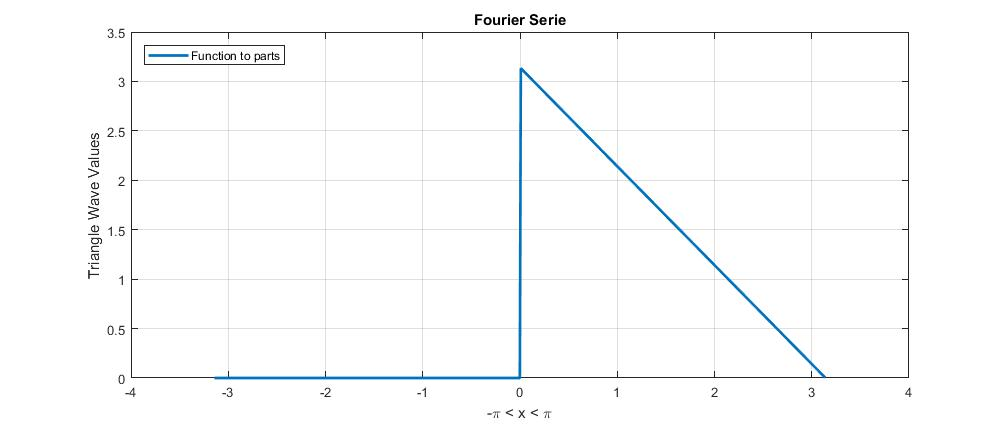
\includegraphics[width=1\textwidth]{n2.jpg}
        \caption{Triangle Wave}
        \label{fig:n2}
    \end{flushright}
\end{figure}

\subsection{Function to parts}
\begin{equation}
    f(t)\begin{Bmatrix}
0 & -\pi< t < 0\\ 
\pi -t & 0 < t <\pi 
\end{Bmatrix}
\quad \text{T= 2$\pi$}
\end{equation}

\subsection{Solution $a_0$}

\begin{equation}
    a_0=\frac{2}{T} \int_{\frac{-T}{2}}^{\frac{T}{2}}f(t)dt = \frac{2}{2 \pi} \int_{\frac{-2 \pi}{2}}^{0}0dt+ \frac{2}{2 \pi} \int_{0}^{\frac{2 \pi}{2}}(\pi - t)dt
\end{equation}

\begin{align*}
    a_0&=\frac{2}{2 \pi} \int_{0}^{\frac{2 \pi}{2}}(\pi - t)dt= \frac{1}{ \pi} \int_{0}^{\pi}(\pi - t)dt\\
    a_0&= \frac{1}{ \pi} \left [\int_{0}^{\pi}\pi dt -  \int_{0}^{\pi}t dt \right ]\\
    a_0&= \frac{1}{ \pi} \left [ \pi t -  \frac{t^2}{2} \right ]_{0}^{\pi}=\frac{1}{ \pi} \left [ \pi (\pi) -  \frac{\pi ^2}{2} \right ]= \frac{1}{ \pi} \left [  \frac{2 \pi^2 -\pi^2}{2} \right ]\\
    a_0&=\frac{1}{ \pi} \left [  \frac{\pi^2}{2} \right ]=\frac{\pi}{2}
\end{align*}

\begin{equation}
\boxed{ a_0=\frac{\pi}{2}}
\end{equation}
\subsection{Solution $a_n$}

\begin{equation}
    a_n=\frac{2}{T} \int_{\frac{-T}{2}}^{\frac{T}{2}}f(t)Cos \left ( \frac{2 n \pi}{T}t\right )dt
\end{equation}

\begin{equation}
    a_n=\frac{2}{2 \pi} \int_{- \pi}^{0}0 \cdot Cos \left ( \frac{2 n \pi}{2 \pi}t\right )dt+\frac{2}{2 \pi} \int_{0}^{\pi}(\pi -x) Cos \left ( \frac{2 n \pi}{2 \pi}t\right )dt
\end{equation}

\begin{align*}
    a&_n=\frac{1}{\pi} \int_{0}^{\pi}(\pi -x)Cos(nt)dt = \frac{1}{\pi}\left [ \int_{0}^{\pi} \pi Cos(nt)dt -tCos(nt)dt \right]\\   
\end{align*}

According to integration tables
\begin{align*}
 \int Cos(nt)dt = \frac{1}{n}Sin(nt)   
\end{align*}

\begin{align*}
   \Aboxed { a_n=\frac{1}{\pi} \left \{\left [\frac{\pi}{n} Sin(nt) \right ]_{0}^{\pi}      - \int_{0}^{\pi} tCos(nt)dt\right \}}
\end{align*}

Integration Methods (Integration by parts)

\begin{equation}
    \int tCos(nt)dt \rightarrow uV- \int V du
\end{equation}

\begin{align*}
    \begin{matrix}
u=t & dv=Cos(nt)dt\\ 
\frac{du}{dt}=1& \int dv =Cos(nt)dt\\ 
 du=dt& V=\frac{1}{n} Sin(nt)
\end{matrix}
\end{align*}

\begin{align*}
    u&V- \int V du \rightarrow t \cdot \frac{1}{n} Sin(nt)- \int \frac{1}{n} Sin(nt)dt\\
   &\frac{t}{n} Sin(nt)- \frac{1}{n} \int  Sin(nt)d \rightarrow  \frac{t}{n} Sin(nt)+ \frac{1}{n^2} Cos(nt)\\
   &a_n=\frac{1}{\pi} \left \{\left [\frac{\pi}{n} Sin(nt) \right ]_{0}^{\pi}      - \left[  \frac{1}{n^2} Cos(nt)+ \frac{t}{n} Sin(nt)\right]_{0}^{\pi}        \right \}\\
   &a_n=\frac{1}{\pi}\left \{ \frac{\pi}{n} Sin(n \pi)- \frac{1}{n^2} Cos(n \pi)-\frac{\pi}{n} Sin(n \pi)+\frac{1}{n^2}  \right \}\\
   Sin(n \pi) =0 \\
    &a_n=\frac{1}{\pi}\left \{ - \frac{1}{n^2} Cos(n \pi)+\frac{1}{n^2}  \right \} = - \frac{1}{\pi n^2} Cos(n \pi)+\frac{1}{\pi n^2}\\
    Cos(n \pi)=(-1)^n\\
    &a_n=\frac{1}{\pi n^2}- \frac{(-1)^n}{\pi n^2}
\end{align*}

\begin{equation}
    \boxed{ a_n=\frac{1-(-1)^n}{\pi n^2}}
\end{equation}

\subsection{Solution $b_n$}

\begin{equation}
    b_n=\frac{2}{T} \int_{\frac{-T}{2}}^{\frac{T}{2}}f(t)Sin \left ( \frac{2 n \pi}{T}t\right )dt
\end{equation}

\begin{equation}
b_n=\frac{2}{2 \pi} \int_{0}^{\frac{2 \pi}{2}}(\pi -t)Sin \left ( \frac{2 n \pi}{2 \pi}t\right )dt=\frac{1}{\pi}\left [ \int_{0}^{\pi} \pi Sin(nt)dt -tSin(nt)dt \right]
\end{equation}

\begin{align*}
b&_n=\frac{1}{\pi}\left [ \int_{0}^{\pi} \pi Sin(nt)dt -\int_{0}^{\pi}tSin(nt)dt \right]\\
&\int tSin(nt)dt=\frac{1}{n^2}Sin(nt)-\frac{t}{n}Cos(nt)\\
&b_n=\frac{1}{\pi}\left [ \frac{-\pi}{n}Cos(nt)-\frac{1}{n^2}Sin(nt)+\frac{t}{n}Cos(nt) \right]_{0}^{\pi}\\
&b_n=\frac{1}{\pi}\left [ \frac{-\pi}{n}Cos(n \pi)+\frac{\pi}{n}-\frac{1}{n^2}Sin(n \pi)+\frac{\pi}{n}Cos(n \pi) \right]\\
Sin(n \pi) =0 \\
\Aboxed{&b_n=\frac{1}{\pi}\left [ \frac{\pi}{n} \right]=\frac{1}{n}}
\end{align*}

\subsection{Coefficients}

\begin{equation}
    \begin{matrix}
a_0=\frac{\pi}{2} &&& a_n=\frac{1-(-1)^n}{\pi n^2} &&&b_n=\frac{1}{n}
\end{matrix}
\end{equation}

\subsection{Replacing coefficients}


\begin{equation}
    f(t)=\frac{\pi}{4}+\sum_{n=1}^{\infty} \left [\frac{1-(-1)^n}{\pi n^2} Cos \left ( \frac{2 n \pi}{T}t\right )  + \frac{1}{n} Sin \left ( \frac{2 n \pi}{T}t\right ) \right ]
\end{equation}

\subsubsection{Evaluation of variable n}

\begin{align*}
    &With\phantom{a}n = 1\\
     &f(t)_{n=1}=\frac{\pi}{4}+\sum_{n=1}^{\infty} \left [\frac{1-(-1)^1}{(\pi) 1^2} Cos \left ( \frac{2 (1) \pi}{2 \pi}t\right )  + \frac{1}{1} Sin \left ( \frac{2 (1) \pi}{2 \pi}t\right ) \right ]\\
     &With\phantom{a}n = 2\\
     &f(t)_{n=2}=\frac{\pi}{4}+\sum_{n=1}^{\infty} \left [  f(t)_{n=1} +\frac{1-(-1)^2}{(\pi) 2^2} Cos \left ( \frac{2 (2) \pi}{2 \pi}t\right )  + \frac{1}{2} Sin \left ( \frac{2 (2) \pi}{2 \pi}t\right ) \right ]\\
     &With\phantom{a}n = 3\\
     &f(t)_{n=3}=...............\\
     &With\phantom{a}n = 4\\
     &f(t)_{n=4}=...............
\end{align*}


\end{document}

